% @Author: Vargas Hector <vargash1>
% @Date:   Saturday, June 25th 2016, 12:52:10 am
% @Email:  vargash1@wit.edu
% @Last modified by:   vargash1
% @Last modified time: Wednesday, June 29th 2016, 8:10:06 pm
\documentclass{article}
%
\usepackage{amsmath}
% Package that is used for units
% Documentation: http://mirror.unl.edu/ctan/macros/latex/contrib/siunitx/siunitx.pdf
\usepackage{siunitx}

% Package used for importing images
\usepackage{graphicx}

% Package used for chemical equations
% Documentation: www.ctan.org/tex-archive/macros/latex/contrib/mhchem/mhchem.pdf
\usepackage[version=3]{mhchem}

% Package used for controlling document margins
\usepackage[margin=1.5in]{geometry}
% Disable page numbering
\pagenumbering{gobble}
% Set relative file path (relative is recommended over  absolute) for image imports
\graphicspath { {./images/} }
% Comments are preceded by %
% LaTeX justifies text by default
\begin{document}
    %----------------------------------------------
    % Cover Page
    % A fancy cover page with centered text
    \thispagestyle{empty}
    % \\ forces a newline
    % \\[1cm]  forces a newline and skips 1cm
    \begin{center}
        % All text in this block is centered
        % Scale image down with .3 factor
        % Note there is no need to include the file extension
        
\includegraphics[scale=0.3]{wit_logo}\\[1cm]
        Exam 1 Writeup using  \LaTeX\\
        Professor G.Sirokman\\
        Hector Vargas\\
        CHEM 1100-4B
    \end{center}
    % Go to new page
    \pagebreak
    %----------------------------------------------

    %%%%%%%%%%%%%%%%%%%%%%%%%%%%%%%%%%%%%%%
    %%%%    ____                   __  %%%%
    %%%%   / __/_ _____ ___ _    <  /  %%%%
    %%%%  / _/ \ \ / _ `/  ' \   / /   %%%%
    %%%% /___//_\_\\_,_/_/_/_/  /_/    %%%%
    %%%%%%%%%%%%%%%%%%%%%%%%%%%%%%%%%%%%%%%

    %----------------------------------------------
    % Question 1 Exam 1
    \begin{center}
        % Bold text
        \textbf{Exam 1 Part 1}\\
        % Italic text
        \textit{Atomic Structure}
    \end{center}
    \textbf{1. There are two naturally occurring types of chlorine, $\ce{^{35}Cl}$ $(34.969 \si{\atomicmassunit})$ and $\ce{^{37}Cl}$ $(36.966 \si{\atomicmassunit})$}

    \textbf{a) Given that the atomic weight of chlorine is $36.45 \si{\atomicmassunit}$, what are the abundances of $\ce{^{35}Cl}$ and $\ce{^{37}Cl}$ ?}

    %You can combine the two to give you italicized bold text
    \textbf{\textit{Solution to a}}
    $$36.45 = 34.969x + 36.966(1 - x)$$
    $$\downarrow$$
    $$x = .759 = 75.9 \%$$

    Thus, $\ce{^{35}Cl}$ accounts for $75.9 \%$ of all chlorine. Whereas $\ce{^{37}Cl}$ accounts for $24.1 \%$ of all chlorine.\\[1cm]

    \textbf{b) What makes $\ce{^{35}Cl}$ different from $\ce{^{37}Cl}$?}

    \textbf{\textit{Solution to b}}

    Both of these isotopes of chlorine differ by the number of neutrons they both have. It's important to note that the number of protons must remain the same. A different number of protons results in a different element. The difference in neutrons is what contributes to the difference in weight.\\[1cm]

    \textbf{c)Which chlorine is regular chlorine and which one is the isotope?}

    \textbf{\textit{Solution to c}}

    The term regular would be a bit inaccurate. They are both regular chlorine, what makes them 'regular' is the fact that one of their isotopes is in higher abundance. Thus $\ce{^{35}Cl}$ is the so called regular chlorine since it is more abundant.
    \pagebreak
    %----------------------------------------------

    %----------------------------------------------
    % Question 2 Exam 1
    \begin{center}
        \textbf{Exam 1 Part 1}\\
        \textit{Unit Analysis}
    \end{center}
    \textbf{2. Consider the two different ways to arrange a large sheet of atoms}

    \textbf{i)How many sulfur atoms(atomic radius $.180 \si{\nano\metre}$) can you fit on a square area $2.5 \si{\micro\metre} * 2.5 \si{\micro\metre}$ in arrangement(a)?}

    \textbf{ii)How many sulfur atoms(atomic radius $.180 \si{\nano\metre}$) can you fit on a square area $2.5 \si{\micro\metre} * 2.5 \si{\micro\metre}$ in arrangement(a)?}

    \textbf{iii)Which of these two layers is denser? By what factor?}

    \pagebreak
    %----------------------------------------------

    %----------------------------------------------
    % Question 3 Exam 1
    \begin{center}
        \textbf{Exam 1 Part 1}\\
        \textit{Atoms}
    \end{center}
    \textbf{3. Consider the modern model of an atom}

    \textbf{a) Draw a diagram of the structure of the atom. Indicate what type of particles exist in each region of the atom.}

    \textbf{\textit{Solution to a}}\\[3cm]

    \textbf{b)Describe the properties of each of the three particles in the atom.}

    \textbf{\textit{Solution to b}}
    \begin{enumerate}
        \item Electrons: Negative charge, amount may be the same as number of Protons
        \item Protons: Positive charge, weight of $1 \si{\atomicmassunit}$, define the element.
        \item Neutrons: No charge, weight of $1 \si{\atomicmassunit}$, define the isotope of the element.\\[1cm]
    \end{enumerate}

    \textbf{c) What is the approximate diameter of an atom?}

    \textbf{\textit{Solution to c}}
    $$ 1 \si{\angstrom} = 1 * 10^{-10} \si{\meter} = .1 \si{\nano\meter} $$
    \pagebreak
    %----------------------------------------------

    %----------------------------------------------
    % Question 4 Exam 1
    %
    \begin{center}
        \textbf{Exam 1 Part 2}\\
        \textit{Acid/Base}
    \end{center}
    \textbf{4. Consider the following questions about acids and bases.}

    \textbf{a) Note for each compound if it is an acid or base. weak or strong}

    \textbf{\textit{Solution to a}}
    \begin{enumerate}
        \item $\ce{NH3}$ Weak Base.
        \item $\ce{HCl}$ Strong Acid.
        \item $\ce{KI}$ Neither an acid or base.
        \item $\ce{Ca(OH)2}$ Strong Base.
    \end{enumerate}

    \textbf{b) Predict the product of the following reaction. Make sure the reaction is balanced.}
    $$\ce{2H3PO4} + \ce{Ca(OH)2} \rightarrow \emptyset + \emptyset$$

    \textbf{\textit{Solution to b}}
    We know that acid base reactions must result in a salt and water. Thus we already know that one of the products is water. Thus the reaction below is what we have so far, all we need now is the salt and balancing. Lets start with the first reactant, balancing tends to rely on even factors.
    $$\ce{2H3PO4} + \ce{Ca(OH)2} \rightarrow \emptyset + \ce{H2O}$$
    Now he have a total of 6 hydrogens, not to mention the 2 hydrogens and 2 oxygens from the 2nd reactant. Thus we know that we have $\ce{8H}$ and $\ce{2O}$. Since one of our products is water, every 2 hydrogen's must have an oxygen.
    $$\ce{2H3PO4} + \ce{3Ca(OH)2} \rightarrow \emptyset + \ce{H2O}$$
    Now we have a total of $\ce{12H}$ and $\ce{6O}$. For each 2 Hydrogens, we have an Oxygen. This gives us.
    $$\ce{2H3PO4} + \ce{3Ca(OH)2} \rightarrow \emptyset + \ce{6H2O}$$
    Now we can much more easily determine the salt.
    $$\ce{2H3PO4}(aq) + \ce{3Ca(OH)2}(aq) \rightarrow \ce{Ca3(PO4)2}(s) + \ce{6H2O}(l)$$

    \textbf{c) Write a net ionic equation for b).}

    \textbf{\textit{Solution to c}}
    $$\ce{6H^{+}} (aq) + \ce{2PO4^{3-}} (aq) + \ce{3Ca^{2+}} (aq) + \ce{6OH^{-}} (aq) \rightarrow \ce{Ca3(PO4)2}(s) + \ce{6H2O}(l)$$

    \textbf{d) Identify the acid and the base in the following reaction(remember the Bronsted Lowry definition)}
    $$\ce{CH_{3}COOH} + \ce{NH_{3}} \rightarrow \ce{CH_{3}COO^{-}} + \ce{NH_{4}^{+}}$$

    \textbf{\textit{Solution to d}}
    According the Bronsted Lowry definition, acids are proton($\ce{H+}$) donators, whereas bases are proton($\ce{H+}$) acceptors. Thus using this definition, we can see that in the above equation that $\ce{CH_{3}COOH}$ was the acid as it lost its hydrogen. This means that $\ce{NH_{3}}$ must be the base.

    \pagebreak

    %----------------------------------------------

    %----------------------------------------------
    % Question 5 Exam 1
    %
    \begin{center}
        \textbf{Exam 1 Part 2}\\
        \textit{Reduction/Oxidation}
    \end{center}
    \textbf{5. In the following reactions}
    \begin{enumerate}
        \item Identify the oxidation state of the elements involved
        \item Indicate what element is being oxidized and what is being reduced
        \item Indicate how many electrons were transferred in the reaction\\[1cm]
    \end{enumerate}

    a) $ \ce{2 C_{2}H_{2}} + \ce{3 O_{2}} \rightarrow \ce{2CO_{2}} + \ce{2 H_{2}O}$

    \textbf{\textit{Solution to a}}
    $$ \ce{2 C_{2}^{-1}H_{2}^{1+}} + \ce{3 O_{2}^{0}} \rightarrow \ce{2C^{4+}O_{2}^{-2}} + \ce{2 H_{2}^{1+}O^{-2}} $$
    Oxygen is being oxidized whereas carbon is being reduced. The amount of electrons transferred in this reaction is
    10. Oxygen has a charge of 0 on the reactant side, but moves on  to have a two -2 charges on the product side. Whereas Carbon loses a total of 6 electrons in order to match the new charge of oxygen on the product side.\\[1cm]

    b) $\ce{Cu^{2+}} + \ce{Zn} \rightarrow  \ce{Zn^{2+}} + \ce{Cu}$

    \textbf{\textit{Solution to b}}
    $$ \ce{Cu^{2+}} + \ce{Zn^{0}} \rightarrow  \ce{Zn^{2+}} + \ce{Cu^{0}} $$
    Copper is being reduced whereas Zinc is being oxidized. The total transfer of electrons is 4. 2 for oxidizing copper from a charge of $+2$ to $0$, and then 2 for reducing zinc from $0$ to $+2$.\\[1cm]

    c) $\ce{P_{4}} + \ce{10 HClO} + \ce{6 H_{2}O} \rightarrow \ce{4 H_{3}PO_{4}} + \ce{10 HCl}$

    \textbf{\textit{Solution to c}}
    $$\ce{P_{4}^{0}} + \ce{10 H^{+1}Cl^{+1}O^{-2}} + \ce{6 H_{2}^{+1}O^{-2}} \rightarrow \ce{4 H_{3}^{+1}PO_{4}^{-3}} + \ce{10 H^{+1}Cl^{-1}}$$
     Phosphorus becomes part of a new compound that has a charge of $-3$, thus it becomes oxidized. Chlorine initially has a charge of $+1$ on the reactant side when it is part of $\ce{HClO}$, however it then becomes reduced in $\ce{HCl}$ by 2 electrons. Thus, the total amount of transferred electrons is 6 electrons.
    \pagebreak
    %----------------------------------------------

    %----------------------------------------------
    % Question 6 Exam 1
    %
    \begin{center}
        \textbf{Exam 1 Part 2}\\
        \textit{Galvanic Series}
    \end{center}
    \textbf{6. You are handed three metal samples. You are told that the three samples are silver, cobalt, and manganese, but that it isn't known which is which. You have available to you some zinc nitrate solution($\ce{Zn(NO3)2}$), nickel nitrate($\ce{Ni(NO3)2}$) solution, and concentrated hydrochloric acid($\ce{HCl}$). Feel free to use the galvanic series below}
    \begin{center}
        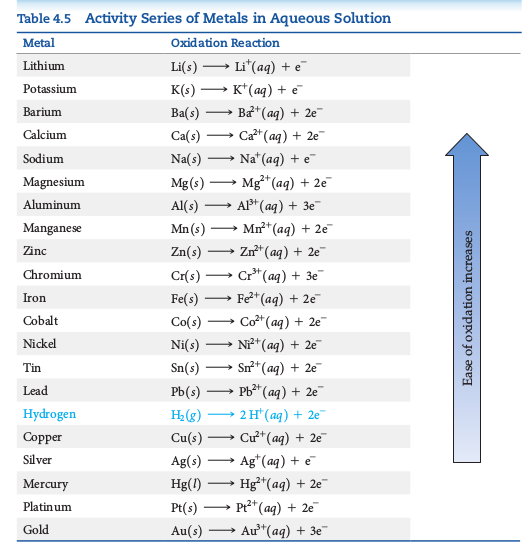
\includegraphics[scale=0.5]{table_4_5}\\[1cm]
    \end{center}
    Describe in detail, with specifics, how you could use the chemicals available to identify the three metal samples. Feel free to make use of the galvanic series below.

    \textbf{\textit{Solution}}

    $\ce{Zn(NO3)2}$ will react with manganese only, you can use this information to identify the manganese sample. $\ce{Ni(NO3)2}$ will react with cobalt and manganese, but since you have identified manganese already, then the solution will react with cobalt only. Thus you have identified 2 of 3 metals. $\ce{HCl}$ will react with all metals except silver, but by process of elimination, you already know silver is the metal that hasn't been identified yet.

    \pagebreak
    %----------------------------------------------

    %----------------------------------------------
    % Question 7 Exam 1
    %
    \begin{center}
        \textbf{Exam 1 Part 3}\\
        \textit{Stoichiometry w/ limiting reagent}
    \end{center}
    \textbf{7. One process used in gold mines to recover gold from mined rock is as shown below}
    $$  \ce{Au} +  \ce{NaCN} +   \ce{O_{2}} +  \ce{H_{2}O} \rightarrow  \ce{NaAu(CN)_{2}} +  \ce{NaOH}$$

    \textbf{a) Balance the reaction}

    \textbf{\textit{Solution to a}}
    $$  \ce{Au} +  \ce{NaCN} +   \ce{O_{2}} +  \ce{2H_{2}O} \rightarrow  \ce{NaAu(CN)_{2}} +  \ce{4NaOH}$$
    $$\downarrow $$
    $$  \ce{Au} +  \ce{8NaCN} +   \ce{O_{2}} +  \ce{2H_{2}O} \rightarrow  \ce{4NaAu(CN)_{2}} +  \ce{4NaOH}$$
    $$\downarrow $$
    $$  \ce{4Au} +  \ce{8NaCN} +   \ce{O_{2}} +  \ce{2H_{2}O} \rightarrow  \ce{4NaAu(CN)_{2}} +  \ce{4NaOH}$$\\[1cm]

    \textbf{b) A small test batch is run in $10 \si{\milli\liter}$($10 \si{\milli\liter}$ is $10 \si{\gram}$ of water). The sample in the reaction contains $0.0178 \si{\gram}$ of gold. It is treated with $0.0115 \si{\gram}$ of $\ce{NaCN}$. $\ce{O_{2}}$ is present in excess. What is the limiting reagent in this test reaction?}

    \textbf{\textit{Solution to b}}
    $$\text{Moles of \ce{Au}} = \dfrac{.0178 \si{\gram}}{197 \si[per-mode=symbol]{\gram\per\mol}} = 9.035 * 10^{-5} \si{\mole}$$
    $$ \text{Moles of \ce{NaCN}} = \dfrac{.0115 \si{\gram}}{49 \si[per-mode=symbol]{\gram\per\mol}} = 2.346 * 10^{-4} \si{\mole}$$
    $$ \text{Moles of \ce{H2O}} = \dfrac{10 \si{\gram}}{18 \si[per-mode=symbol]{\gram\per\mol}} = 0.555 \si{\mole}$$
    Our limiting reactant is gold as expected.\\[1cm]

    \textbf{c) What mass of $\ce{NaAu(CN)_{2}}$ would be produced by the    reaction described by b?}

    \textbf{\textit{Solution to c}}

    Since we know gold is our limiting reactant and the reaction is $\ce{4 Au}$ : $\ce{4NaAu(CN)2}$.

    $$ \text{Grams of \ce{NaAu(CN)2}} = 9.035 * 10^{-5} \si{\mole} * 272 \si[per-mode=symbol]{\gram\per\mol} = .0245  \si{\gram}$$

    \pagebreak
    %----------------------------------------------

    %----------------------------------------------
    % Question 8 Exam 1
    %
    \begin{center}
        \textbf{Exam 1 Part 3}\\
        \textit{Stoichiometry With Story}
    \end{center}
    \textbf{8. Back in the day, aluminum was a highly precious metal. It was first isolated in the early 1800s. It's synthesis involved the reaction of aluminum chloride with potassium}
    $$ \ce{3K} + \ce{AlCl3} \rightarrow \ce{Al} + \ce{3KCl}$$

    The Baron Von Markov has decided that he wants a full aluminum place setting, and you have been pout in charge of making the required aluminum. You have to produce $520 \si{\gram}$ of aluminum using the reaction shown above, which work in $87\%$ yield. How much aluminum chloride($\ce{AlCl_{3}}$) and potassium($\ce{K}$) will you need to be able to produce the needed amount of aluminum?

    \textbf{\textit{Solution}}
    $$ \text{Moles of \ce{Al}} = \dfrac{520 \si{\gram}}{27 \si[per-mode=symbol]{\gram\per\mol}} = 19.26 \si{\mole}$$
    $$\downarrow$$
    $$ \text{Moles of \ce{K}} = 19.26 \si{\mole} * 3 = 57.78 \si{\mole} $$
    $$ \text{Moles of \ce{AlCl3}} = 19.26 \si{\mole} * 1 = 19.26 \si{\mole} $$
    $$\downarrow$$
    $$ \text{Mass of \ce{K}} = 57.78 \si{\mole} * 39 \si[per-mode=symbol]{\gram\per\mol} = 2252.25 \si{\gram}$$
    $$ \text{Mass of \ce{AlCl3}} = 19.26 \si{\mole} * 132 \si[per-mode=symbol]{\gram\per\mol} = 2542.32 \si{\gram} $$

    \pagebreak
    %----------------------------------------------

    %----------------------------------------------
    % Question 9 Exam 1
    %
    \begin{center}
        \textbf{Exam 1 Part 3}\\
        \textit{Stoichiometry With Solutions Chemistry}
    \end{center}
    \textbf{9. Early lighter than air balloons often used hydrogen gas for lift. This hydrogen gas was generally produced from the reaction of iron and sulfuric acid as shown here:}
    $$\ce{Fe} + \ce{H_{2}SO_{4}} \rightarrow \ce{FeSO_{4}} + \ce{H_{2}}$$

    \textbf{a) Is this reaction an acid base reaction or an oxidation reduction reaction(or neither?). Justify your answer.}

    \textbf{\textit{Solution to a}}

    This reaction is a redox reaction, Fe has a charge of 0 on the reactant side, yet has a charge of $2+$ of the product side.\\[1cm]

    \textbf{b) In a test reaction, reacting $100 \si{\gram}$ of iron with excess sulfuric acid produced $1.45 \si{\mole}$ of hydrogen gas. What is the percent yield of this reaction?}

    \textbf{\textit{Solution to b}}
    $$\text{Moles of \ce{Fe}} = \dfrac{100 \si{\gram}}{ 56 \si[per-mode=symbol]{\gram\per\mol}} = 1.785 \si{\mole}$$
    $$\text{Theoretical \ce{H} Yield} = 1.785 * 2 \si[per-mode=symbol]{\gram\per\mol} = 3.571 \si{\gram}  = 1.785 \si{\mole} \text{ of Hydrogen}$$
    $$\text{Percent Yield} = \dfrac{\text{Actual}}{\text{Theoretical}} = \dfrac{1.45}{1.785} * 100\% = 81.23 \%$$\\[1cm]

    \textbf{c) A balloon with the volume of $100 \si{\liter}$ needs to be filled with hydrogen. How much iron and sulfuric acid will be needed to produce the required amount of hydrogen gas to fill the $100 \si{\liter}$ balloon? To help, 1 $\si{\mole}$ of gas fills $24 \si{\liter}$ of volume. \textbf{Make sure to account for the yield calculated in b!}}

    \textbf{\textit{Solution to c}}
    $$\dfrac{100 \si{\liter}}{24 \si{\liter}} = 4.16 \si{\mole} \text{ of gas needed} $$
    Accounting for yield
    $$\text{Actual} = \dfrac{4.16}{x} = .83 = 5.012 \si{\mole} $$
    $$\text{Moles of \ce{Fe} and \ce{H2SO4} needed} = 5.012 \si{\mole} $$
    $$\text{Mass of \ce{Fe} needed} =  5.012 \si{\mole} * 56 \si[per-mode=symbol]{\gram\per\mol} = 280.67 \si{\gram}$$
    $$\text{Mass of \ce{H2SO4} needed} =  5.012 \si{\mole} *   98 \si[per-mode=symbol]{\gram\per\mol} = 491.17 \si{\gram}$$

    \pagebreak
    %----------------------------------------------

    %----------------------------------------------
    % Bonus Exam 1
    %
    \begin{center}
        \textbf{Exam 1 Bonus}\\
    \end{center}

    \textbf{A) Describe the phenomenon due to which the region of the atmosphere we call the sky is blue at noon on a sunny day. (aka Why is the sky blue?)}

    \textbf{Solution}

    Blue light is the type of light most scattered by air. At dawn and dusk, the angle of the light from the sun causes more red to be scattered near the sun. Which is why we see reddish sunsets and sunrises.\\[1cm]

    \textbf{B) We have talked about two ways to categorize compounds so far, molecules, and ionic compounds. How are these two types of compounds different from each other? How does difference influence the way they behave in solution?}

    \textbf{Solution}

    These two different types of compounds primarily differ in the method in which they bond. Ionic compounds transfer electrons, whereas molecules share electrons. Ionic compounds will require transfer of electrons to react in a solution, whereas compounds will require you to break their bonds.

    \pagebreak
    %----------------------------------------------

    %----------------------------------------------
    % Cover Page
    \thispagestyle{empty}
    \begin{center}
        
\includegraphics[scale=0.3]{wit_logo}\\[1cm]
        Exam 2 Writeup using  \LaTeX\\
        Professor G.Sirokman\\
        Hector Vargas\\
        CHEM 1100-4B
    \end{center}
    \pagebreak
    %----------------------------------------------

    %----------------------------------------------

    %%%%%%%%%%%%%%%%%%%%%%%%%%%%%%%%%%%%%%%
    %%%%    ____                  ____ %%%%
    %%%%   / __/_ _____ ___ _    |_  | %%%%
    %%%%  / _/ \ \ / _ `/  ' \  / __/  %%%%
    %%%% /___//_\_\\_,_/_/_/_/ /____/  %%%%
    %%%%%%%%%%%%%%%%%%%%%%%%%%%%%%%%%%%%%%%

    %----------------------------------------------
    % Question 1 Exam 2
    %
    \begin{center}
        \textbf{Exam 2 Part 1}\\
        \textit{Stoichiometry}
    \end{center}
    \textbf{1. The spores of the hive mind have just landed on a planet, and you have begun your hungry search for more raw matter to build a new hive cluster. OF special interest to you are local minerals, which are predominantly unobtanium trioxide ($\ce{UbO_{3}}$). The stars in the Koprulu sector are capable of making super heavy atoms, so unobtanium($\ce{Ub}$) has an atomic weight of $558 \dfrac{\si{\gram}}{\si{\mol}}$}

    You need to hatch some Zerglings fast to kill some of the more violent local fauna, like the human farmers over the next hill. A zergling egg requires $400 \si{\kilo\gram}$ of pure unobtanium to produce, and each egg hatches two zerglings. Carbon(readily available) and unobtanium trioxide react to form unobtanium and carbon dioxide. This reaction has a yield of $85\%$ for unobtanium.

    How many kilograms of minerals and how many kilograms of carbon do you need to make 10 zerglings?

    \textbf{Solution}

    Before we begin, it should already be quite evident that Unobtanium is our limiting reagent as carbon is readily available.
    $$ \ce{2UbO3} + \ce{3C} \rightarrow \ce{2Ub} + \ce{3CO2}$$
    $$ \text{Molar Mass(\ce{UbO3})} = 606 \si[per-mode=symbol]{\gram\per\mole} \quad \text{Molar Mass(\ce{Ub})} = 558 \si[per-mode=symbol]{\gram\per\mole}  $$
    $$2000 \si{\kilo\gram} \, \ce{Ub} \text{ Required for 10 eggs} $$
    $$\text{Moles of \ce{Ub} required} = \dfrac{2000 \si{\kilo\gram}}{558 \si[per-mode=symbol]{\gram\per\mole}} = 3584.23 \si{\mole}$$
    This is under $100\%$ yield conditions however, we must correct this.
    $$\dfrac{3584.23}{x} = .85 \rightarrow x = 4216.74 \si{\mole} \text{ Actual Yield}$$
    $$\text{Mass(\ce{UbO3})} = (4216.74 \si{\mol}) * 606 \si[per-mode=symbol]{\gram\per\mole} = 2555344.44 \si{\gram} $$
    Since we know reactant is a $2:3$ ratio.
    $$\text{Mass(\ce{C})} = 2555344.44 \si{\gram} * \dfrac{3}{2} = 3833016.66 \si{\gram}$$
    \pagebreak
    %----------------------------------------------

    %----------------------------------------------
    % Question 2 Exam 2
    %
    \begin{center}
        \textbf{Exam 2 Part 1}\\
        \textit{Unit Analysis}
    \end{center}
    \textbf{2. Consider the two different ways to arrange a large sheet of atoms}

    i) How many gold atoms(atomic radius $.144 \si{\nano\metre}$) can you fit on a square area $1.5 \si{\micro\metre} * 1.5 \si{\micro\metre}$ in arrangement(a)?

    ii) How many gold atoms(atomic radius $.144 \si{\nano\metre}$) can you fit on a square area $1.5 \si{\micro\metre} * 1.5 \si{\micro\metre}$ in arrangement(a)?

    iii) Calculate the density $(\dfrac{\text{mass}}{\text{volume}})$ of a single atom layer of arrangement a)

    \pagebreak
    %----------------------------------------------

    %----------------------------------------------
    % Question 3 Exam 2
    %
    \begin{center}
        \textbf{Exam 2 Part 1}\\
        \textit{Red/Ox}
    \end{center}
    \textbf{3. Jewelers have numerous tests to be able to tell whether a piece of jewelry is fake. For instance, lead is often used in making fake gold items. A jeweler is handed a gold ring, but is suspicious as to whether it is gold or not. He uses a tool to make a tiny scratch on the surface of the ring, and drips some concentrated hydrochloric acid($\ce{H^{+}}$) on it. He then observes that bubbles are formed in the acid solution. Use the table below to explain the chemistry that was observed if the ring was made of lead.}
    \begin{center}
        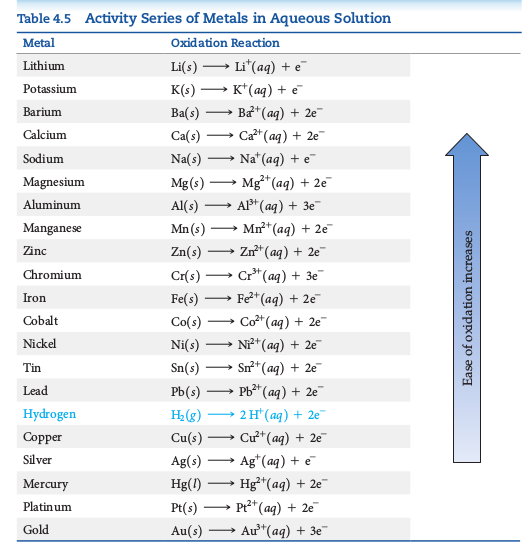
\includegraphics[scale=0.35]{table_4_5}\\[1cm]
    \end{center}

    \textbf{Solution to a}

    According to the galvanic series in the table, lead will react with the hydrochloric acid. Gold, Silver, Platinum, and Gold will not! Thus if bubbles form, then the piece of metal he is holding is not precious. Please call the police.

    \textbf{Although gold is not damaged by hydrochloric acid, it can be corroded by aqua regia, a mixture of nitric acid and hydrochloric acid. Below is the reaction between gold and aqua regia. Confirm that it is a red/ox reaction. Identify what element is oxidized and what is reduced. Indicate how many electrons are transferred.}
    $$\ce{Au}(s) + \ce{HNO_{3}}(aq) + \ce{4 HCl}(aq) \rightarrow \ce{HAuCl_{4}}(aq) + \ce{2 H2O}(l) + \ce{NO}(g)$$

    \textbf{Solution to b}
    $$\ce{Au}(s) + \ce{H^{+1}NO_{3}^{-1}}(aq) + \ce{4 H^{+1}Cl^{-1}}(aq) \rightarrow \ce{H^{+1}Au^{+3}Cl_{4}^{-1}}(aq) + \ce{2 H2O}(l) + \ce{NO}(g)$$
    We can see that the gold is being oxidized and gaining 3 electrons. $\ce{NO3}$ is the element that is being reduced. There are the electrons that were transferred in the reaction.
    \pagebreak
    %----------------------------------------------

    %----------------------------------------------
    % Question 4 Exam 2
    %
    \begin{center}
        \textbf{Exam 2 Part 2}\\
        \textit{Photon Energies}
    \end{center}
    \textbf{4. The Imperial Star Destroyer, His Left Hand, has departed space dock and is cruising around Tatooine. It spots the Rebel Frigatte, Valorous, and opens fire. His Left Hand's turbo laser batteries fires lasers with photons of wavelength $551 \si{\nano\meter}$.}

    \textbf{a) If \textit{Valorous} is hit by a $10 \si{\mega\joule}$ blast of energy from the laster fire, how many photons hit the Valorous?}

    $$ h = 6.626 * 10^{-34} \si{\joule} \cdot \si{\second}$$
    $$ c = 3.00 * 10^{8} \frac{\si{\meter}}{\si{\second}} $$

    \textbf{Solution to a}
    $$ E_{\text{photon}} = \dfrac{hc}{5.51 * 10^{-7} \si{\meter}} = 3.8900196 * 10^{-19} \si{\joule} $$
    $$ \text{Number of Photons} = \dfrac{10\si{\mega\joule}}{3.8900196 * 10^{-19} \si{\joule}} = 2.5707 * 10^{25}$$\\[1cm]

    \textbf{b) \textit{His Left Hand} is using a copper based laser emitter. What is happening inside the copper atoms to emit photons?}

    \textbf{Solution to b}

    Electrons that are excited will move to a higher energy level, when they drop back down to their ground state. Photons are emitted. This is known as an elements light emission spectrum.
    \pagebreak
    %----------------------------------------------

    %----------------------------------------------
    % Question 5 Exam 2
    %
    \begin{center}
        \textbf{Exam 2 Part 2}\\
        \textit{Electron Configuration}
    \end{center}
    \textbf{5. Consider the following questions relating to electron configurations of atoms.}

    a) Write the electron configurations of the following elements:
    \begin{enumerate}
        \item S\\
        \textbf{Solution: }
        $[\ce{Ne}]3s^{2}3p^{4}$
        \item N\\
        \textbf{Solution: }
        $[\ce{He}]2s^{2}2p^{3}$
    \end{enumerate}

    b) Draw an energy diagram for the electron configuration of oxygen (with lines for each orbital and electrons as arrows). What ion is the most likely ion that oxygen will form? Explain based on your electron configuration.
    \textbf{Solution to b: }\\[3cm]


    c) Using quantum numbers, explain why the $n = 2$ shell has an $s$ and $p$ sub shell but no $d$ or $f$ sub shells.

    \textbf{Solution to c: }

    It wouldn't be able to fit them. At the $n = 2$ shell, sub shells $1s$, $2s$, and $2p$ can exist. Technically at $n = 2$, 4 orbitals can exist. The $1s$ and $2s$ sub shell each have one orbital and then 2 more orbitals are in the $2p$ sub shell. It's worth mentioning that both the $1s$ and $2s$ shell can each hold 2 electrons. The $2p$ shell can hold 6 however.

    \pagebreak
    %----------------------------------------------

    %----------------------------------------------
    % Question 6 Exam 2
    %
    \begin{center}
        \textbf{Exam 2 Part 2}\\
        \textit{Orbitals}
    \end{center}
    \textbf{6. Consider the following questions relating to electron configurations of atoms.}

    a)Draw a digram, showing the probability of finding the electron on the $y$ axis, and distance from the nucleus on the $x$ axis for a $2s$ orbital\\[2cm]

    b)Draw a diagram, showing the probability of finding the electron on the $y$ axis, and distance from the nucleus on the $x$ axis for a $2p$ orbital.\\[2cm]

    c)Draw a picture of a $2p$ orbital\\[2cm]

    d)In your diagrams and pictures above. Indicate the locations of any nodes. How many nodes does each type of orbital have?

    Each type of orbital has one node.\\[2cm]

    e)What appears to be a common theme between $2s$ and $2p$ orbitals based on your answers in d?

    Same amount of nodes, node closer to nucleus.
    \pagebreak
    %----------------------------------------------

    %----------------------------------------------
    % Question 7 Exam 2
    %
    \begin{center}
        \textbf{Exam 2 Part 3}\\
        \textit{Atomic Size}
    \end{center}
    \textbf{7. Consider the following questions relating to atomic size and lattice energy.}

    \textbf{a) Put the following sets of atoms in order of increasing size and \textit{explain} your choice for ordering}
    $$\ce{O}, \ce{N}, \ce{F}, \ce{C}$$

    \textbf{Solution to a}

    A trend regarding atomic size is observable from the periodic table. As we go the right of the table, atoms get smaller. As we go to the bottom, atoms get bigger. Thus in order from smallest to largest, $\ce{F}$, $\ce{O}$, $\ce{N}$, $\ce{C}$.
    One such explanation to this is the electron count that these elements have. In the same order, electron count goes from largest to smallest. More electrons result in a greater pull towards the nucleus, which leads to the pattern in size.\\[1cm]

    \textbf{b) There are two components to changes in lattice energies. The values below are an example of each. What is suggested by each trend? What changes appear to have the greater influence on lattice energy? Explain in detail.}
    \begin{enumerate}
        \item $\ce{LiF}$ $1060 \dfrac{\si{\kilo\joule}}{\si{\mole}} \qquad$ $\ce{CsI}$  $600 \dfrac{\si{\kilo\joule}}{\si{\mole}}$
        \item  $\ce{LiF}$ $1060 \dfrac{\si{\kilo\joule}}{\si{\mole}} \qquad$ $\ce{MgO}$  $3900 \dfrac{\si{\kilo\joule}}{\si{\mole}}$
    \end{enumerate}

    \textbf{Solution to b}

    1. $\ce{LiF}$ has a greater lattice energy due to the size difference. The increased atomic radii of $\ce{Cs}$ and $\ce{I}$ results in less lattice energy. Lithium and Fluorine are smaller relative to Cesium and Iodine, resulting in a tighter pull from the nucleus to the electrons. Thus, $\ce{LiF}_{\text{Lattice Energy}} > \ce{CsI}_{\text{Lattice Energy}}$

    2. In contrary to the previous question. The charge of each element has more influence on the lattice energy. $\ce{Mg^{2+}}$ and $\ce{O^{2-}}$ have a greater net charge difference than $\ce{Li^{+}}$ and $\ce{F^{-}}$
    \pagebreak
    %----------------------------------------------

    %----------------------------------------------
    % Question 8 Exam 2
    %
    \begin{center}
        \textbf{Exam 2 Part 3}\\
        \textit{Bond Enthalpy}
    \end{center}
    \textbf{8. Currently the vast majority of commercially used hydrogen is generated according to the following reaction.}
    $$\ce{CH4} + \ce{2H2O} \rightarrow \ce{CO2} + \ce{4H2}$$
    \begin{center}
        $\ce{C-H}$ $413 \frac{\si{\kilo\joule}}{\si{\mol}} \quad$
        $\ce{C-O}$ $358 \frac{\si{\kilo\joule}}{\si{\mol}} \quad$
        $\ce{O-O}$ $146 \frac{\si{\kilo\joule}}{\si{\mol}} \quad$
        $\ce{C=O}$ $799 \frac{\si{\kilo\joule}}{\si{\mol}}$\\[.2cm]
        $\ce{O-H}$ $463 \frac{\si{\kilo\joule}}{\si{\mol}} \quad$
        $\ce{C-C}$ $348 \frac{\si{\kilo\joule}}{\si{\mol}} \quad$
        $\ce{O=O}$ $495 \frac{\si{\kilo\joule}}{\si{\mol}} \quad$
        $\ce{H-H}$ $436 \frac{\si{\kilo\joule}}{\si{\mol}}$
    \end{center}

    a) What is the enthalpy change($\Delta H$) for this reaction per $\ce{CO2}$? Is energy released or absorbed?

    \textbf{Solution to a}
    $$ \Delta = (4(413) + 2(2(463))) - (2(799) + 4(436)) = 162 \si[per-mode=symbol]{\kilo\joule\per\mole}$$
    Energy is absorbed

    b) There are a variety of means of recovering energy from $\ce{H2}$, either from giving heat through combustion or electricity electrochemically from a fuel cell. What is the energy released in this reaction?
    $$\ce{2H2} + \ce{O2} \rightarrow \ce{2H2O}$$

    \textbf{Solution to b}

    $$\Delta = (2(436) + (495)) - 2(2(463))  = -485 \si[per-mode=symbol]{\kilo\joule\per\mole}$$

    c) Combining a) and b), do some stoichiometry to find the net energy released per $\ce{CO2}$ produced.

    \textbf{Solution to c}

    Net energy released per $\ce{CO2}$, $\Delta = 799 * 2 = 1598 \si[per-mode=symbol]{\kilo\joule\per\mole}$

    \pagebreak
    %----------------------------------------------

    %----------------------------------------------
    % Question 9 Exam 2
    %
    \begin{center}
        \textbf{Exam 2 Part 3}\\
        \textit{Bond Polarity}
    \end{center}
    \textbf{8. Consider the following questions about bonding and polarity.}

    a) Order the following bonds from most to least polar. Show your calculations.
    \begin{enumerate}
        \item $\ce{Na-Cl}$ in $\ce{NaCl}$ $\quad \Delta EN = 2.1$ Ionic
        \item $\ce{B-F}$ in $\ce{BF3}$ $\quad \Delta EN = 2.0$ Ionic
        \item $\ce{O-H}$ in $\ce{H2O}$ $\quad \Delta EN = 1.4$ Polar covalent
        \item $\ce{Cl-H}$ in $\ce{HCl}$ $\quad \Delta EN = 0.9$ Polar covalent
        \item $\ce{F-F}$ in $\ce{F2}$ $\quad \Delta EN = 0$ Non polar covalent
        \item $\ce{S=C}$ in $\ce{CS2}$ $\quad \Delta EN = 0$ Non polar covalent
    \end{enumerate}

    c) What does it mean for a bond to be polar? How is this different from a bond being ionic?

    For a bond to be polar, the electrons that are shared within the molecule tend to sway more to one side than the other. This isn't the same as an ionic bond, where electrons quite literally transfer from one element to the other.
    \pagebreak
    %----------------------------------------------

    %----------------------------------------------
    % Bonus Exam 2
    %
    \begin{center}
        \textbf{Exam 2 Bonus}\\
    \end{center}

    A) Describe the phenomenon due to which the region of the atmosphere we call the sky is blue at noon on a sunny day. (aka Why is the sky blue?)

    Blue light is the type of light most scattered by air. At dawn and dusk, the angle of the light from the sun causes more red to be scattered near the sun. Which is why we see reddish sunsets and sunrises.\\[1cm]

    B) Use Molecular Orbitals to explain whether or not $\ce{He2+}$ molecule should be able to exist.

    \textbf{Answer}\\
    $$\text{Bond Order} = \dfrac{2 - 0}{2} = 1$$
    It would be reasonable for $\ce{He2+}$ to exist. A bond order of 0 would suggest it's too unstable.

    \pagebreak
    %----------------------------------------------

    %%%%%%%%%%%%%%%%%%%%%%%%%%%%%%%%%%%%%%%
    %%%%    ____                  ____ %%%%
    %%%%   / __/_ _____ ___ _    |_  / %%%%
    %%%%  / _/ \ \ / _ `/  ' \  _/_ <  %%%%
    %%%% /___//_\_\\_,_/_/_/_/ /____/  %%%%
    %%%%%%%%%%%%%%%%%%%%%%%%%%%%%%%%%%%%%%%

    %----------------------------------------------
    % Cover Page
    \thispagestyle{empty}
    \begin{center}
        
\includegraphics[scale=0.3]{wit_logo}\\[1cm]
        Exam 3 Writeup using  \LaTeX\\
        Professor G.Sirokman\\
        Hector Vargas\\
        CHEM 1100-4B
    \end{center}
    \pagebreak
    %----------------------------------------------

    %----------------------------------------------
    % Question 1 Exam 3
    %
    \begin{center}
        \textbf{Exam 3 Part 1}\\
        \textit{Stoichiometry}
    \end{center}
    \textbf{1. When hydrogen sulfide gas ($\ce{H2S}$) is bubbled into a solution of sodium hydroxide ($\ce{NaOH}$), the reaction forms sodium sulfide ($\ce{Na2S}$) and water. How many grams of sodium sulfide are formed if $3.50 \si{\gram}$ of hydrogen sulfide is bubbled into a solutions containing $4.20 \si{\gram}$ of sodium hydroxide, assuming that the sodium sulfide is made in $73\%$ yield?.}

    $$\ce{H2S} + \ce{2NaOH} \rightarrow \ce{Na2S} + \ce{2H2O}$$
    $$\text{Moles of \ce{H2S}} = \dfrac{3.50 \si{\gram}}{34 \si[per-mode=symbol]{\gram\per\mole}} = 0.103 \si{\mol}$$
    $$\text{Moles of \ce{NaOH}} = \dfrac{4.20 \si{\gram}}{40 \si[per-mode=symbol]{\gram\per\mole}} = 0.105 \si{\mol}$$

    We know that 1 mole of $\ce{H2S}$ requires 2 of $\ce{NaOH}$, thus the base is our limiting reagent.

    $$.105 \si{\mol} \div 2 =  .0525 \si{\mol} \ce{Na2S}$$

    However now we need to consider the $73 \%$ yield.

    $$.73 = \dfrac{x}{.0535}$$
    $$x = .038 \si{\mol} $$

    Now all we do is multiply $\ce{Na2S}$ molar mass by our calculated mole amount after yield:
    $$.038 \si{\mol} * 78 \si[per-mode=symbol]{\gram\per\mole} = 2.964 \si{\gram} $$
    Thus we have produced $ 2.964 \si{\gram}$ of $\ce{Na2S}$
    \pagebreak
    %----------------------------------------------

    %----------------------------------------------
    % Question 2 Exam 3
    %
    \begin{center}
        \textbf{Exam 3 Part 1}\\
        \textit{Spectral Lines}
    \end{center}
    \textbf{2. The Rydberg equation can be used to predict the spectral emissions of hydrogen atoms. $R_{H} = 1.097 * 10^{7}  \si{\meter^{-1}}$; $c = 3.00 * 10^{8} \si[per-mode=symbol]{\meter\per\second}$; $h = 6.626 * 10^{-34} \si{\joule} \si{\second}$.}

    \textbf{a)  The Balmer series is the series of emissions arising from the fall of an electron from a higher orbital to the $n = 2$ orbital. Calculate the wavelength of the lowest energy transition in the Balmer series.}\\
    \textbf{\textit{Solution}}
    $$\dfrac{1}{\lambda} = R_{H}(\dfrac{1}{n^{2}_{f}} - \dfrac{1}{n^{2}_{i}}) \rightarrow \dfrac{1}{\lambda} = R_{H}(\dfrac{1}{2^{2}} - \dfrac{1}{3^{2}})$$
    $$\downarrow$$
    $$\dfrac{1}{\lambda} = 1523611.11^{-1} \rightarrow \lambda = 656 \si{\nano\metre}$$
    It's important to note that this wavelength is well within our viewing range!

    \textbf{b) The Lyman series is a set of emissions arising from the fall of an electron from a higher orbital to the $n = 1$ orbital. Do you expect emissions in this series to be higher in energy or lower than the Balmer series? Explain.}\\
    \textbf{\textit{Solution}}
    $$\dfrac{1}{\lambda} = R_{H}(\dfrac{1}{1^{2}} - \dfrac{1}{2^{2}}) \rightarrow 1.215 * 10^{-7} = 121 \si{\nano\meter}$$
    $$E = \dfrac{hc}{\lambda} $$
    $$ \downarrow $$
    $$E_{656 \si{\nano\meter}} = \dfrac{hc}{6.56 * 10^{-7}}  = 3.030 * 10^{-19} \si{\joule}$$
    $$E_{121 \si{\nano\meter}} = \dfrac{hc}{1.215 * 10^{-7}} = 1.636 * 10^{-18} \si{\joule}$$

    Shorter wavelengths have higher energy. Which is why gamma rays are dangerous, but transitions from higher orbital to lowest increase in energy. Such as $n=5$ to $n=2$. Thus, these emissions would be higher. The real contributor to more energy is higher $n$ orbital drop.

    \pagebreak
    %----------------------------------------------

    %----------------------------------------------
    % Question 3 Exam 3
    %
    \begin{center}
        \textbf{Exam 3 Part 1}\\
        \textit{Bond Enthalpy}
    \end{center}
    \textbf{4. Ethanol is a common additive to gasoline nowadays. Ethanol, however, is said to be less energy dense.\\ Here are a few energy bonds:}
    \begin{center}
        $\ce{C-H}$ $413 \  \si[per-mode=symbol]{\kilo\joule\per\mol} \quad$
        $\ce{C-O}$ $358 \ \si[per-mode=symbol]{\kilo\joule\per\mol} \quad$
        $\ce{O-O}$ $146 \  \si[per-mode=symbol]{\kilo\joule\per\mol} \quad$
        $\ce{C=O}$ $799 \  \si[per-mode=symbol]{\kilo\joule\per\mol}$\\[.2cm]
        $\ce{O-H}$ $463 \  \si[per-mode=symbol]{\kilo\joule\per\mol} \quad$
        $\ce{C-C}$ $348 \  \si[per-mode=symbol]{\kilo\joule\per\mol} \quad$
        $\ce{O=O}$ $495 \  \si[per-mode=symbol]{\kilo\joule\per\mol}$
    \end{center}

    \textbf{a) How much energy is released per mole of ethanol($\ce{C2H5OH}$)?}
    $$(5(413) + 348 + 358 + 463 + 3(495)) - (2(2*799) + 3(2*463))  = 1255 \si{\kilo\joule\per\mole}$$

    \textbf{b) How much energy is released per liter of ethanol burnt?(density = $.789 \si[per-mode=symbol]{\gram\per\milli\liter}$)?}
    $$\text{Mass of ethanol in 1 Liter}  = 1000 \si{\milli\liter} * .789 \si[per-mode=symbol]{\gram\per\milli\liter}  = 789 \si{\gram} $$
    $$\text{Molar mass of ethanol} = 46 \si[per-mode=symbol]{\gram\per\mole} $$
    $$789 \si{\gram} \div 46 \si[per-mode=symbol]{\gram\per\mole} = 17.152 \si{\mol}$$
    $$1255 \si[per-mode=symbol]{\kilo\joule\per\mole} * 17.152 \si{\mol}  = 21525.76 \si{\kilo\joule}$$
    Which is a lot of energy released.
    \pagebreak
    %----------------------------------------------

    %----------------------------------------------
    % Question 4 Exam 3
    %
    \begin{center}
        \textbf{Exam 3 Part 2}\\
        \textit{MO Theory}
    \end{center}
    \textbf{4.}

    \textbf{a) Draw a molecular orbital digram for the molecule $\ce{F2}$}\\[2cm]

    \textbf{b) What is the Bond Order of $\ce{F2}$(show calculations)? Does this match what is predicted by Lewis structures(You will have to draw a Lewis structure to convince me)?}
    $$ \dfrac{10 - 8}{2} = 1$$
    $$ \ce{F-F}$$

    \textbf{c) Is $\ce{F2}$ diamagnetic or paramagnetic? How will it react to a magnetic field?}

    $\ce{F2}$ is paramagnetic due to a set of  unpaired electrons, it will be attracted to a magnetic field.
    \pagebreak
    %----------------------------------------------

    %----------------------------------------------
    % Question 5 Exam 3
    %
    \begin{center}
        \textbf{Exam 3 Part 2}\\
        \textit{Heating Curves}
    \end{center}
    \textbf{5. \textit{Valorous}, the rebel frigate is having a luck day. \textit{His Left Hand's} (Imperical Cruiser) shields are down, so a $15 \si{\giga\joule}$ blast of energy hits the side of the ship. Let us assume that this ship was made with low grade materials like steel(we'll approximate it's characteristics with iron). Calculate what the maximum amount of steel/iron this shot could vaporize is. Assume the side of the ship is at $300 \si{\kelvin}$ due to the heat generated inside the Cruiser. The melting point of iron is $1811 \si{\kelvin}$, the boiling point is $3134 \si{\kelvin}$, the specific heat of solid iron is $.445 \si[per-mode=symbol]{\joule\per\gram\kelvin}$. The specific heat of liquid iron is $.611 \si[per-mode=symbol]{\joule\per\gram\kelvin}$, the heat of fusion for iron is $13.8 \si[per-mode=symbol]{\kilo\joule\per\mole}$ and the heat of vaporization for iron is $340 \si[per-mode=symbol]{\kilo\joule\per\mole}$. Build a strategy to solve the problem. As one option, try to find the energy to boil a small amount of the material and go from there.}

    Using a $1000 \si{\kilo\gram}$ sample of iron to begin with.
    $$E_{1} = (.445 \si[per-mode=symbol]{\joule\per\gram\kelvin})(1000 \si{\gram})(1811 - 300 \si{\kelvin})  = 672395 \si{\joule}$$
    $$E_{2} = (13800 \si[per-mode=symbol]{\joule\per\mole})(1000 \si{\gram} \div 56 \si[per-mode=symbol]{\gram\per\mole}) = 246428.57 \si{\joule}$$
    $$E_{3} = (.611 \si[per-mode=symbol]{\joule\per\gram\kelvin})( 2.10 * 10^{6} \si{\gram})(3134 - 1811 \si{\kelvin})  = 1697541300 \si{\joule}$$
    $$E_{4} = (340000 \si[per-mode=symbol]{\joule\per\mole})(2.10 * 10^{6} \si{\gram} \div 56 \si[per-mode=symbol]{\gram\per\mole}) = 1.275 * 10^{10} \si{\joule}$$

    This sums up to roughly $1.44 * 10^{10} \si{\joule}$, a bit short of $1.5 * 10^{10} \si{\joule}$. The total amount that we were able to vaporize with this amount is $2.10 * 10^{6} \si{\gram} + 1000 \si{\gram} $
    They way I came about this is once I got to $E_{3}$, I stopped and subtracted the used energy from the 15 Gigajoules available. The equation looked like this. A bit short, but since this number is so big, it will be in the same magnitude as the actual solution.

    $$(.611 \si[per-mode=symbol]{\joule\per\gram\kelvin})( x \si{\gram})(3134 - 1811 \si{\kelvin})  =  340000 *(x \div 56) \approx 2.10*10^{6}$$


    \pagebreak
    %----------------------------------------------

    %----------------------------------------------
    % Question 6 Exam 3
    %
    \begin{center}
        \textbf{Exam 3 Part 2}\\
        \textit{Molecular Orbitals}
    \end{center}
    \textbf{6. Below is a presented the molecular orbital diagram for $\ce{Li2}$}

    \textbf{a) What is the bond order for this molecule?}

    \textbf{\textit{Solution}}
    $$\text{Bond Order} = \dfrac{4 - 2}{2} = 1$$

    \textbf{b) Which of the molecular orbitals will have nodal planes? What does this imply about these orbitals(the ones with nodal planes?)}

    $2s$ has a nodal plane, you are not likely to find an electron within these nodes. This suggest that the likelihood of finding an electron within these planes is pretty much 0.

    \textbf{c) The $\ce{Li2}$ molecule is hit by a photon, and one of the $\sigma_{2s}$ electrons is promoted to the $\sigma_{2s}^{*}$ orbital. Would this be a stable molecule? }

    \textbf{\textit{Solution}}
    $$\text{New Bond Order} = \dfrac{2 - 2}{2} = 0$$
    The bond order is now 0, this leads to the molecule being unstable and rather unlikely to exist.

    \textbf{d) The strength of a $\ce{Li-Li}$ bond in $\ce{Li2}$ is $215 \si[per-mode=symbol]{\kilo\joule\per\mole}$. What is the wavelength of the photon in question c?}
    $$ c = 3.0 * 10^{8} \si[per-mode=symbol]{\meter\per\second} \quad h = 6.626 * 10^{-34} \si{\joule\second}$$

    $$\dfrac{1}{\lambda} = R_{H}(\dfrac{1}{1^{2}} - \dfrac{1}{2^{2}}) = 1.215436 * 10^{-7} \si{\meter} $$

    \pagebreak
    %----------------------------------------------

    %----------------------------------------------
    % Question 7 Exam 3
    %
    \begin{center}
        \textbf{Exam 3 Part 3}\\
        \textit{Acids/Bases}
    \end{center}
    \textbf{7.}

    \textbf{a) What is the pH of a $.0034 M$ solution of         $\ce{NaOH}$?}

    $$pH = 14 - (-1 * \log_{10}(.0034)) = 11.53 $$

    \textbf{b) What is the pH of a $.0034 M$ solution of         $\ce{CH3COOH}$? ($k_{a} = 1.8 * 10^{-5}$)}
    $$\ce{CH3COOH <=> CH3COO- + H+}$$

    $$1.8 * 10^{-5} = \dfrac{\ce{[CH3COO^{-}]}{\ce{[H^{+}]}}}{[\ce{CH3COOH}]} $$
    $$1.8 * 10^{-5} = \dfrac{x^{2}}{.0034 - x} $$
    \textbf{c) what is the pH of a solution made from equal volumes of the solutions in a and b?(Consider what you are starting off with after the two solutions react. Same as $k_{a}$ as above applies.)}
    $$\ce{CH3COOH + OH- <=> CH3COO- + H2O}$$
    $$1.8 * 10^{-5} = \dfrac{\ce{[CH3COO^{-}]}{\ce{[H2O]}}}{[\ce{CH3COOH}][\ce{OH^{-}}]} $$


    \pagebreak
    %----------------------------------------------

    %----------------------------------------------
    % Question 8 Exam 3
    %
    \begin{center}
        \textbf{Exam 3 Part 3}\\
        \textit{Intermolecvular Forces}
    \end{center}
    \textbf{8. Consider the following questions about Van Der Waals forces.(Hint Draw lewis structures)}

    \textbf{a) Ethane $(\ce{C2H6})$ and formaldehyde ($\ce{CH2O}$) have the same molar mass and similar size. Formaldehyde, however, boils at $-19\,^{\circ}\mathrm{C}$, and ethane boils at $-89\,^{\circ}\mathrm{C}$. Explain this difference in terms of intermolecular forces.}

    The difference in boiling point suggests that formaldehyde has a particular type of intermolecular force that ethane does not have. Ethane's lewis structure is simply 2 carbons surrounded by hydrogen. Thus, it has no dipole-dipole interaction. We know that all compounds have London dispersion forces, thus it leaves us with Formaldehyde either having dipole-dipole attractions or h-bonds. However, formaldehyde cannot have h-bonds as it does not meet the criteria for doing so. Thus we know that formaldehyde has dipole-dipole intermolecular forces while ethane does not.  We can confirm this with the usage of Lewis structures. As you can see, the oxygen's charge is the primary reason for the dipole-dipole charge.

    \textbf{b) Methane $(\ce{CH4})$ and water ($\ce{H2O}$) have the same molar mass and similar size. None the less, methane boils at $-161\,^{\circ}\mathrm{C}$  whereas water boils at $100\,^{\circ}\mathrm{C}$. Explain this  dramatic difference in terms of intermolecular forces.}

    Unlike Methane, water has a hydrogen bond. These types of bonds are much stronger than London dispersion forces and dipole-dipole forces. Methane only has London dispersion forces, similar to Ethane in the previous example. This would explain why $\ce{HF}$ is known for having such a strong bond.
    \pagebreak
    %----------------------------------------------

    %----------------------------------------------
    % Question 9 Exam 3
    %
    \begin{center}
        \textbf{Exam 3 Part 3}\\
        \textit{Equilibrium}
    \end{center}
    \textbf{9. Consider the reactions:}
    $$ \ce{2NO} (\si{\gram}) \ce{<=>} \ce{N2}(\si{\gram}) + \ce{O2}(\si{\gram})$$
    $$\text{The K of the reaction is } 2.4*10^{3} \text{ at }  2000\,^{\circ}\mathrm{C}$$

    If $0.256 \si{\mole}$ of $\ce{NO}$ is introduced into a $1.35 \si{\liter}$ reactor and is allowed to come to equilibrium what will be the final concentrations of $\ce{NO }$, $\ce{N2}$, and $\ce{O2}$ be?

    \pagebreak
    %----------------------------------------------


\end{document}
